\documentclass[8pt]{beamer}
\usetheme[secheader]{pecostalk}
\graphicspath{{figs/}}
%\usepackage{comment}
\newcommand{\paramred}[1]{{\color{red} #1}}
\newcommand{\measblue}[1]{{\color{blue} #1}}
\newcommand{\bgamma}{\bar{\gamma}}
\newcommand{\GRINS}{\texttt{GRINS}}
\newcommand{\libMesh}{\texttt{libMesh}}
\definecolor{darkgreen}{rgb}{0,0.4,0}

\setbeamerfont{normal text}{size=\small}


\title[Model Inadequacy in Supercapacitors]{
DiaMond\\
{\small Model Inadequacy in Models of Supercapacitors}
}
%\subtitle{}

\author[Moser et al]{
Robert Moser,\\ 
Danial Faghihi,
Todd Oliver,
Damien Lebrun-Grandie
$~$\\
{\small
Institute for Computational Engineering and Sciences (ICES)\\
$\quad~$The University of Texas at Austin
}
}

\date[DiaMond October 2016]{
{\it DiaMond XXXXX,
October XX, 2016
}
}

\begin{document}


%===============================================================================
% Slide 1
%===============================================================================
\begin{frame}
\frametitle{Models of Supercapacitors}
\vfill

%\vspace{0.05in}
\begin{itemize}

\item $\eta(\xi,\tau)$ = overpotential in electrode: $\eta = \phi_{solid}-\phi_{liquid}-U_{eq}$\\
\item $\gamma$ = conductivity ratio of solid and liquid \\
\item $\xi, \tau$ = dimensionless distance and time \\
\item $I(\tau)$ = applied current

\end{itemize}
\vspace{-0.1in}
\begin{columns}
\begin{column}{.47\textwidth}
%-----------------------------
\begin{block}{High Fidelity (1D) model}
\vspace{-0.05in}
\begin{equation*}\label{eq:HF}
\frac{\partial\eta_{HF}}{\partial\tau} = \frac{\partial^2\eta_{HF}}{\partial\xi^2}
\end{equation*}
\vspace{-0.1in}
\begin{small}
\begin{equation*}
\left\{\begin{matrix}
\frac{\partial\eta_{HF}}{\partial\xi}|_{\xi=0} & = & -\frac{\gamma}{1+\gamma}I(\tau)\\
\frac{\partial\eta_{HF}}{\partial\xi}|_{\xi=1} & = & \frac{1}{1+\gamma}I(\tau) \nonumber\\
\eta_{HF}|_{\tau=0} 					       & =  & \eta_0(\xi)
\end{matrix}\right.
\end{equation*}
\end{small}
\vspace{-0.05in}
\end{block}
%-----------------------------
\vspace{-0.08in}
\begin{block}{Low Fidelity (0D) model}
%\begin{footnotesize}
 \vspace{-0.15in}
\begin{eqnarray*}\label{eq:LF}
\eta_{LF} = \frac{1}{2}I\xi^2- I \frac{\gamma}{1+\gamma}\xi + {\eta}^{avg}(\tau)
			 - I\frac{2\gamma-1}{6(1+\gamma)}
	\vspace{-0.3in}		 
\end{eqnarray*}
%\vspace{-0.1in}
where $\frac{\partial{\eta}^{avg}}{\partial\tau} = I$
%\vspace{-0.1in}
%\end{footnotesize}
\end{block}
%-----------------------------
\end{column}
%====================
\begin{column}{.5\textwidth}
\begin{center}
\vspace{-0.35in}
\begin{figure}[h]
    \centering
%    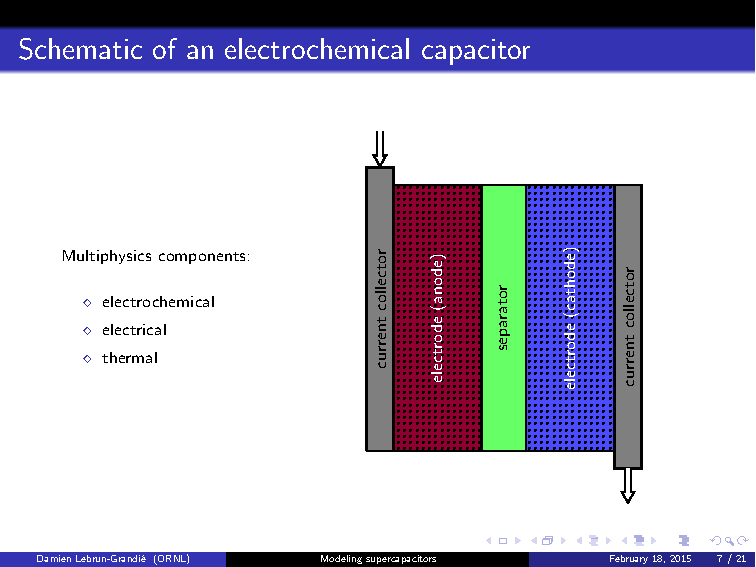
\includegraphics[trim = 2.4in 0.4in 0.7in 0.9in, clip, width=.3\textwidth]{figs_report/supercap_schematic.pdf}
%    \\    \vspace{0.02in} 
    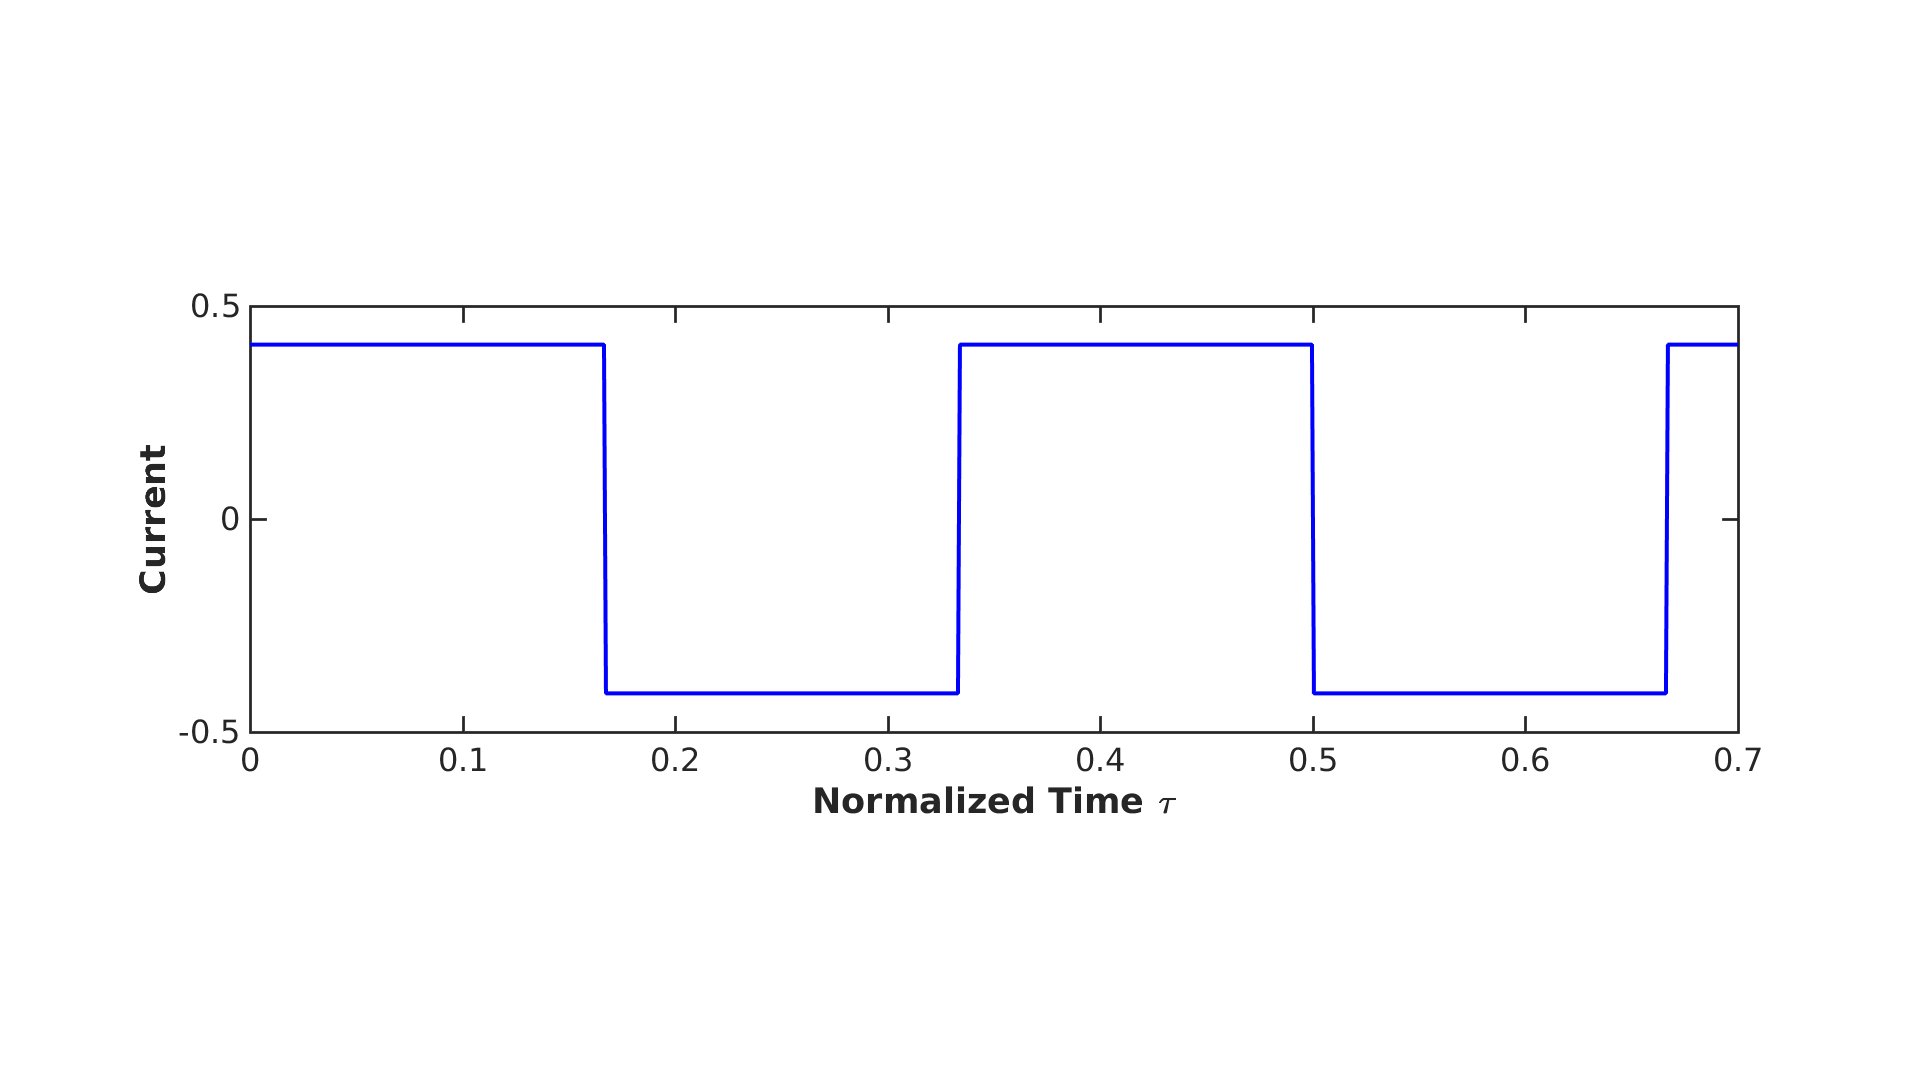
\includegraphics[trim = 1.2in 2.4in 1.6in 2.8in, clip, width=0.95\textwidth]{figs_report/I.png}
    \\
    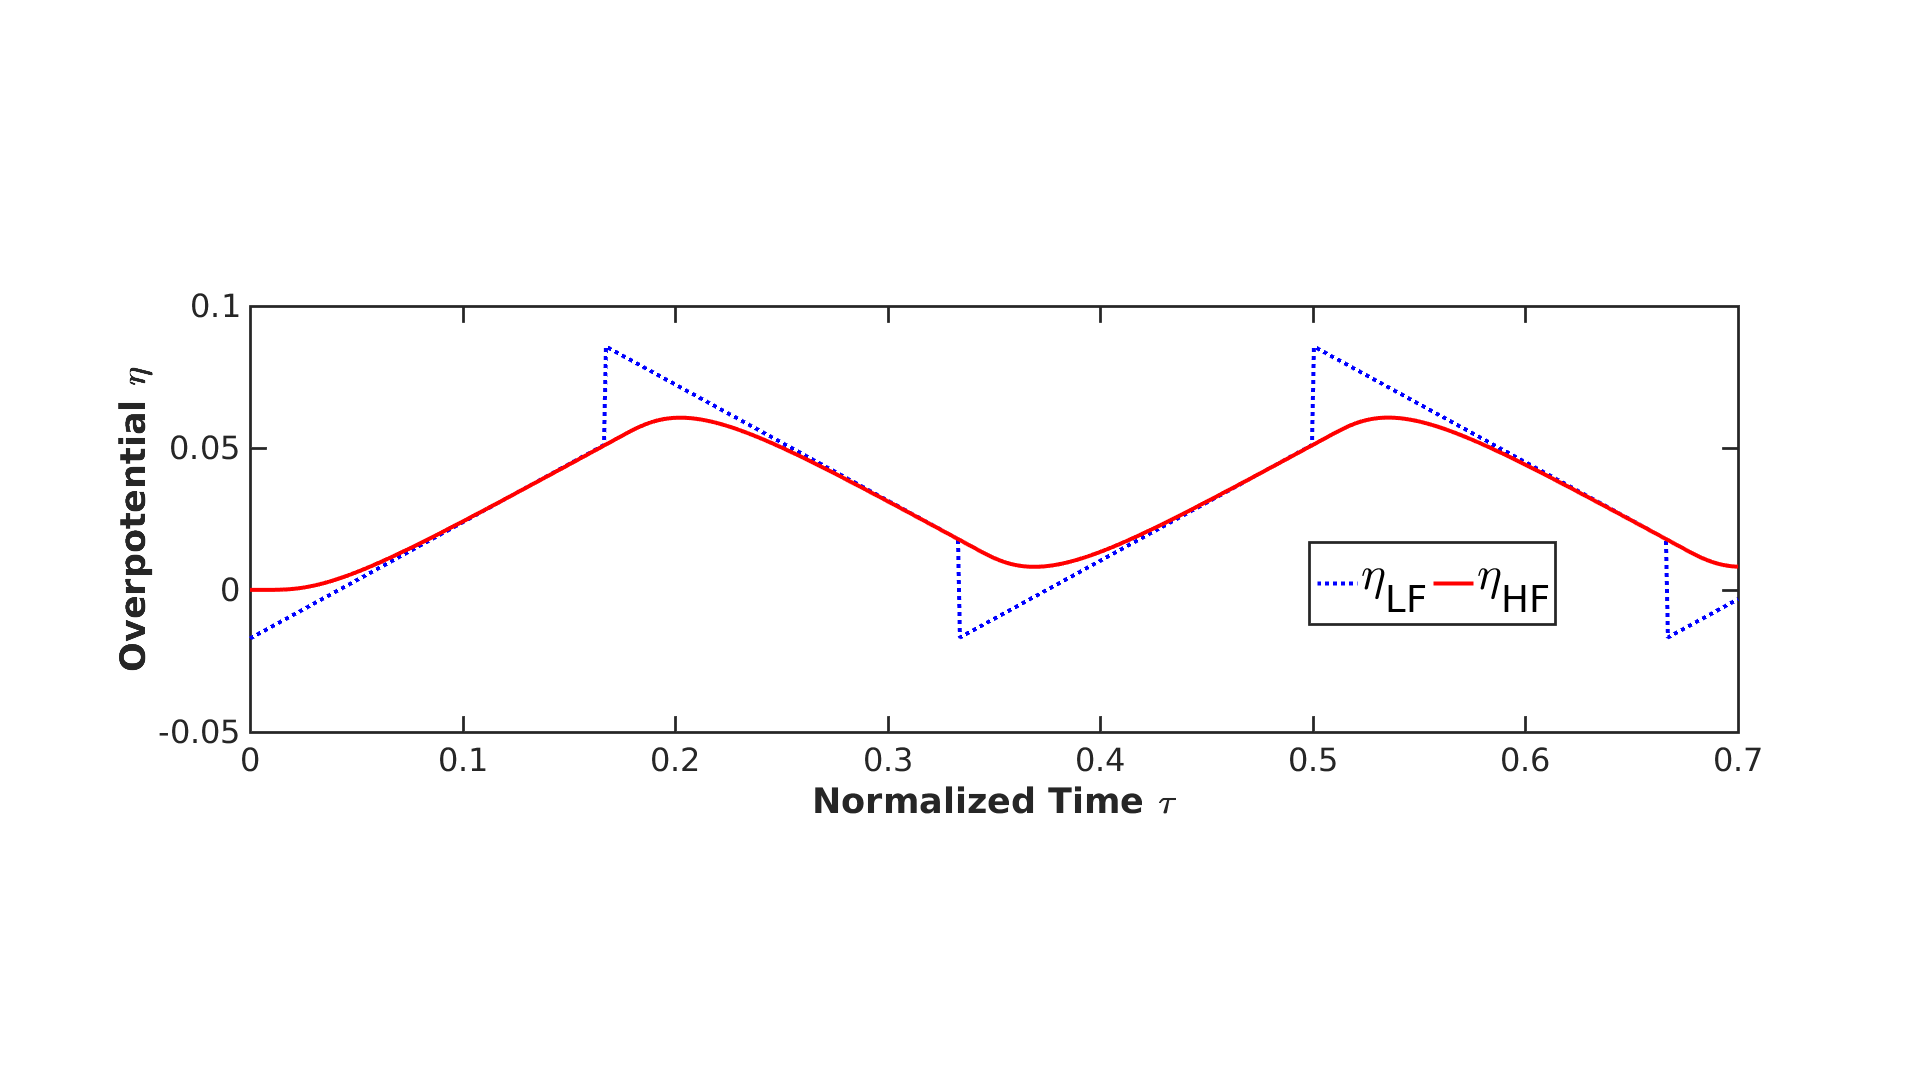
\includegraphics[trim = 1.2in 2.4in 1.6in 2.8in, clip, width=0.95\textwidth]{figs_report/etaLF_HF.png}   
    \\
    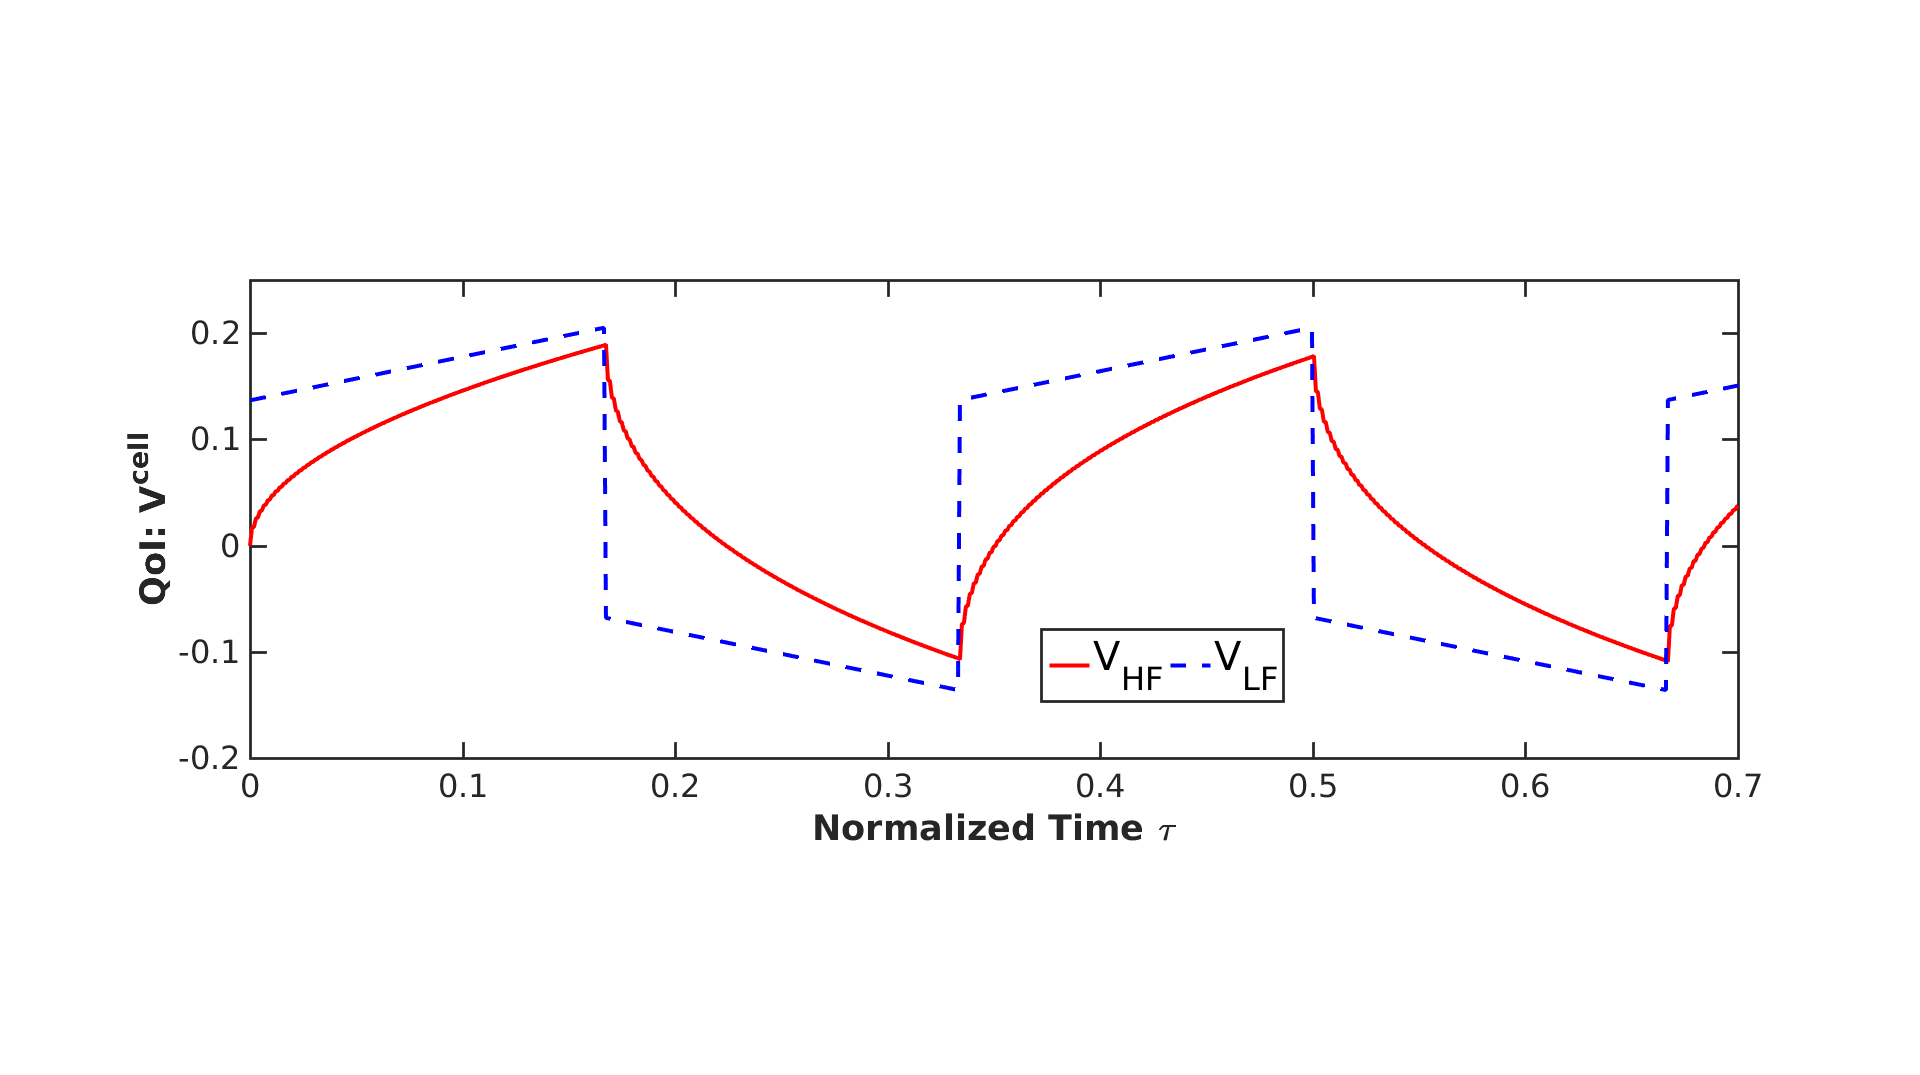
\includegraphics[trim = 1.2in 2.4in 1.6in 2.8in, clip, width=0.95\textwidth]{figs_report/Vcell_HF_LF.png} 
\end{figure}
\end{center}
\end{column}
\end{columns}
%====================
\vspace{-0.05in}
\begin{columns}
\begin{column}{.65\textwidth}
\begin{alertblock}{Quantity of Interest}
 Potential drop across the system
 
 $V^{cell}(\tau) = \phi_{collector}^L - \phi_{collector}^R
= \frac{1+2\gamma}{1+\gamma}\eta|_{\xi=1} - \frac{\gamma}{1+\gamma}\eta|_{\xi=0} - \frac{\gamma}{(1+\gamma)^2}I
 $
\end{alertblock} 
\end{column}
%====================
\begin{column}{.3\textwidth} 
    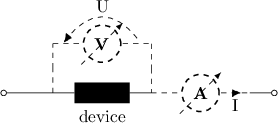
\includegraphics[trim = 0in 0in 0.in 0.2in, clip, width=0.95\textwidth]{figs_report/device.png}
\end{column}
\end{columns}



\vfill
\end{frame}

%===============================================================================
% Slide 2
%===============================================================================
\begin{frame}
\frametitle{Model Inadequacy}
\vfill

\vspace{0.1in}
\begin{itemize}
\item The high fidelity model accounts for the time history of the current. Such history does not appear with right dependency in the low fidelity model: 
%
\begin{small}
\begin{eqnarray*}
V^{cell}_{HF} =& A(\gamma)\int_0^{\tau} I(\tau') K(\tau-\tau') d\tau' &+ B(\gamma) I(\tau)\\
V^{cell}_{LF} =& C(\gamma)\int_0^{\tau} I(\tau') d\tau' &+ D(\gamma) I(\tau)
\end{eqnarray*}
\end{small}
\item The stochastic inadequacy representation needs to account for the incomplete and uncertain history information available to the low-fidelity model.
\item Solution of low fidelity model converges to high fidelity over time i.e. modeling error is larger for higher frequency current. 
%\item Given what we know about high fidelity model $\eta_{HF}$, one can formulate inadequacy representation. 
\end{itemize}

\vspace{0.in}
\begin{columns}
\begin{column}{.44\textwidth}
%-----------------------------
\vspace{-0.05in}
\begin{alertblock}{Inadequacy representation}

\begin{center}
Error in QoI: \quad
$\epsilon = V^{cell}_{HF} - V^{cell}_{LF}$
\end{center}
\vspace{-0.05in}
\textbf{Auxiliary Stochastic ODE:}
\begin{equation*}
\frac{\partial\epsilon}{\partial\tau} = -\lambda\epsilon + \alpha \frac{\partial I}{\partial\tau}
\end{equation*}

where $\lambda$ is a stochastic process with following time evolution:
\begin{equation*}
\frac{\partial\lambda}{\partial\tau} = -c(\lambda - \lambda_{mean}) + \beta \frac{\partial W}{\partial\tau}
\end{equation*}

where $W(\tau)$ is a Wiener process.% and $(\alpha, \beta, c, \lambda_{mean})$ are parameters of inadequacy representation. 
\end{alertblock}

\end{column}
%====================
\begin{column}{.52\textwidth}
\begin{center}
%\vspace{-4mm}
\begin{figure}[h]
    \centering
    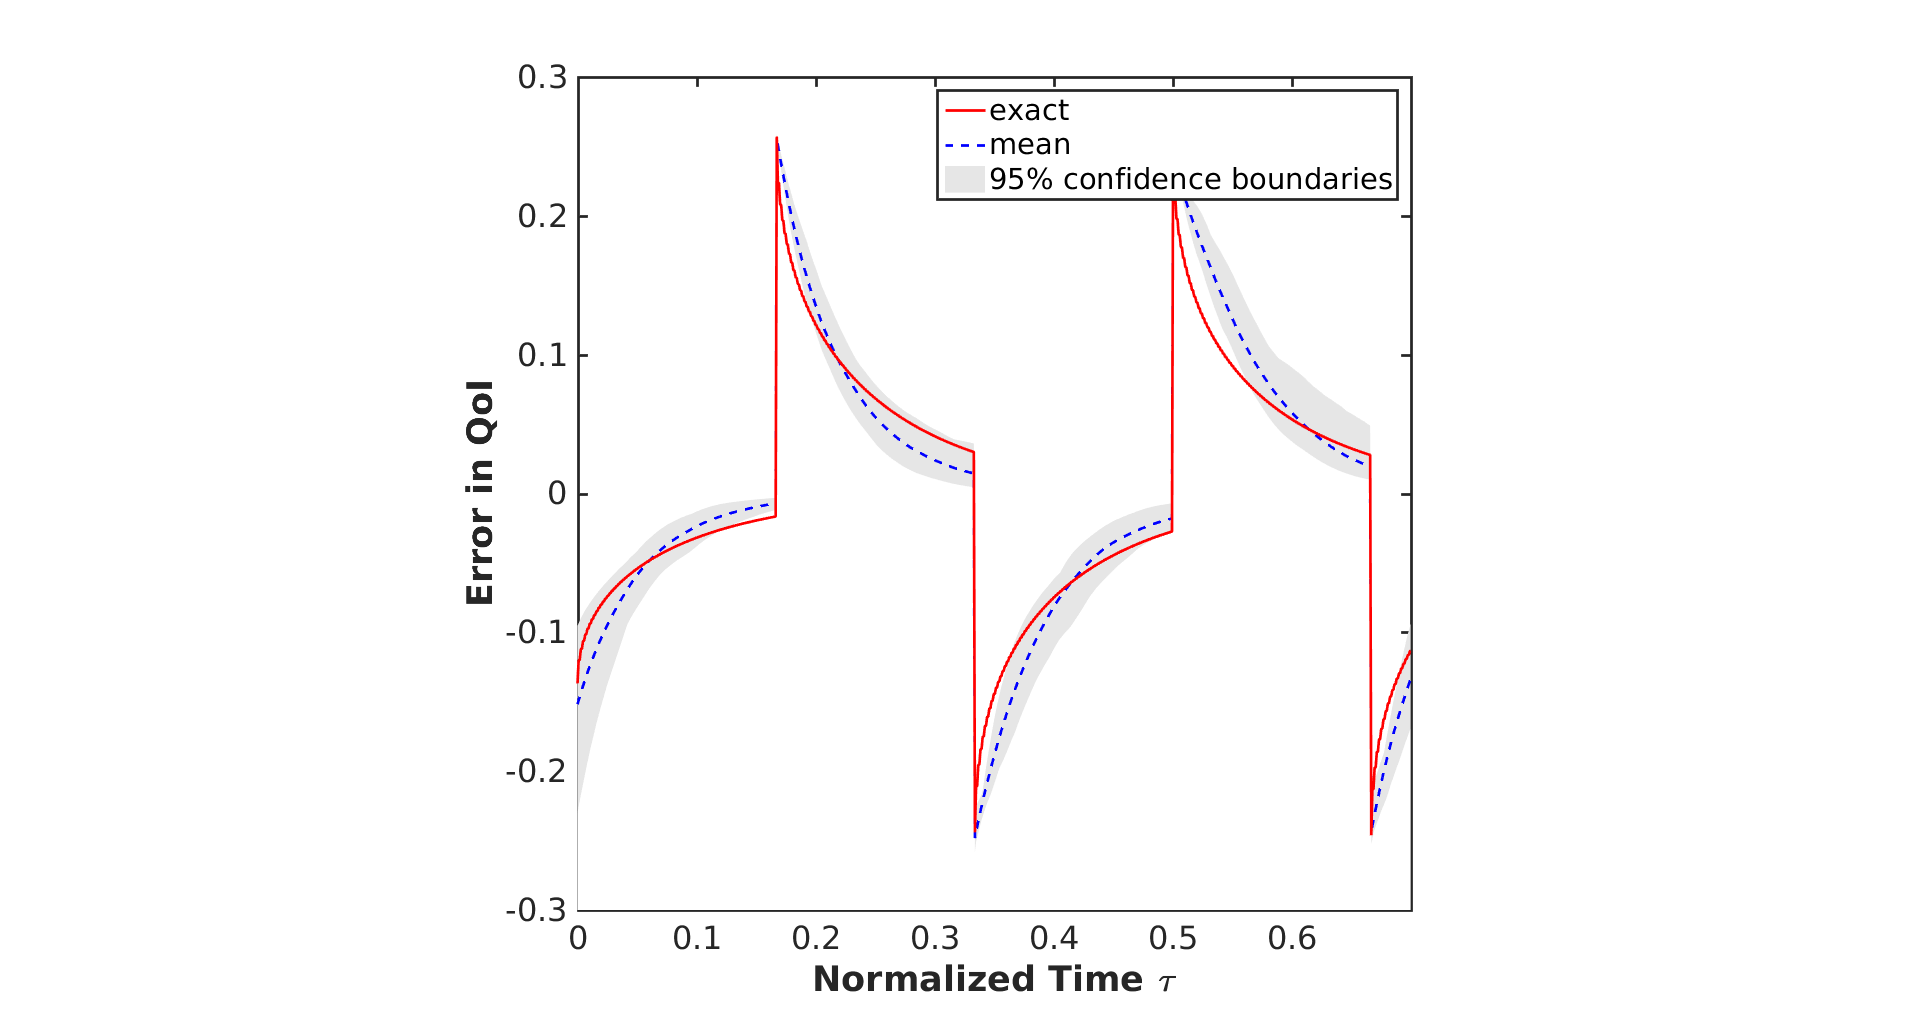
\includegraphics[trim = 1.3in 2.2in 1.6in 2.8in, clip, width=1\textwidth]{figs_report/error_bound.png} 
        \\
    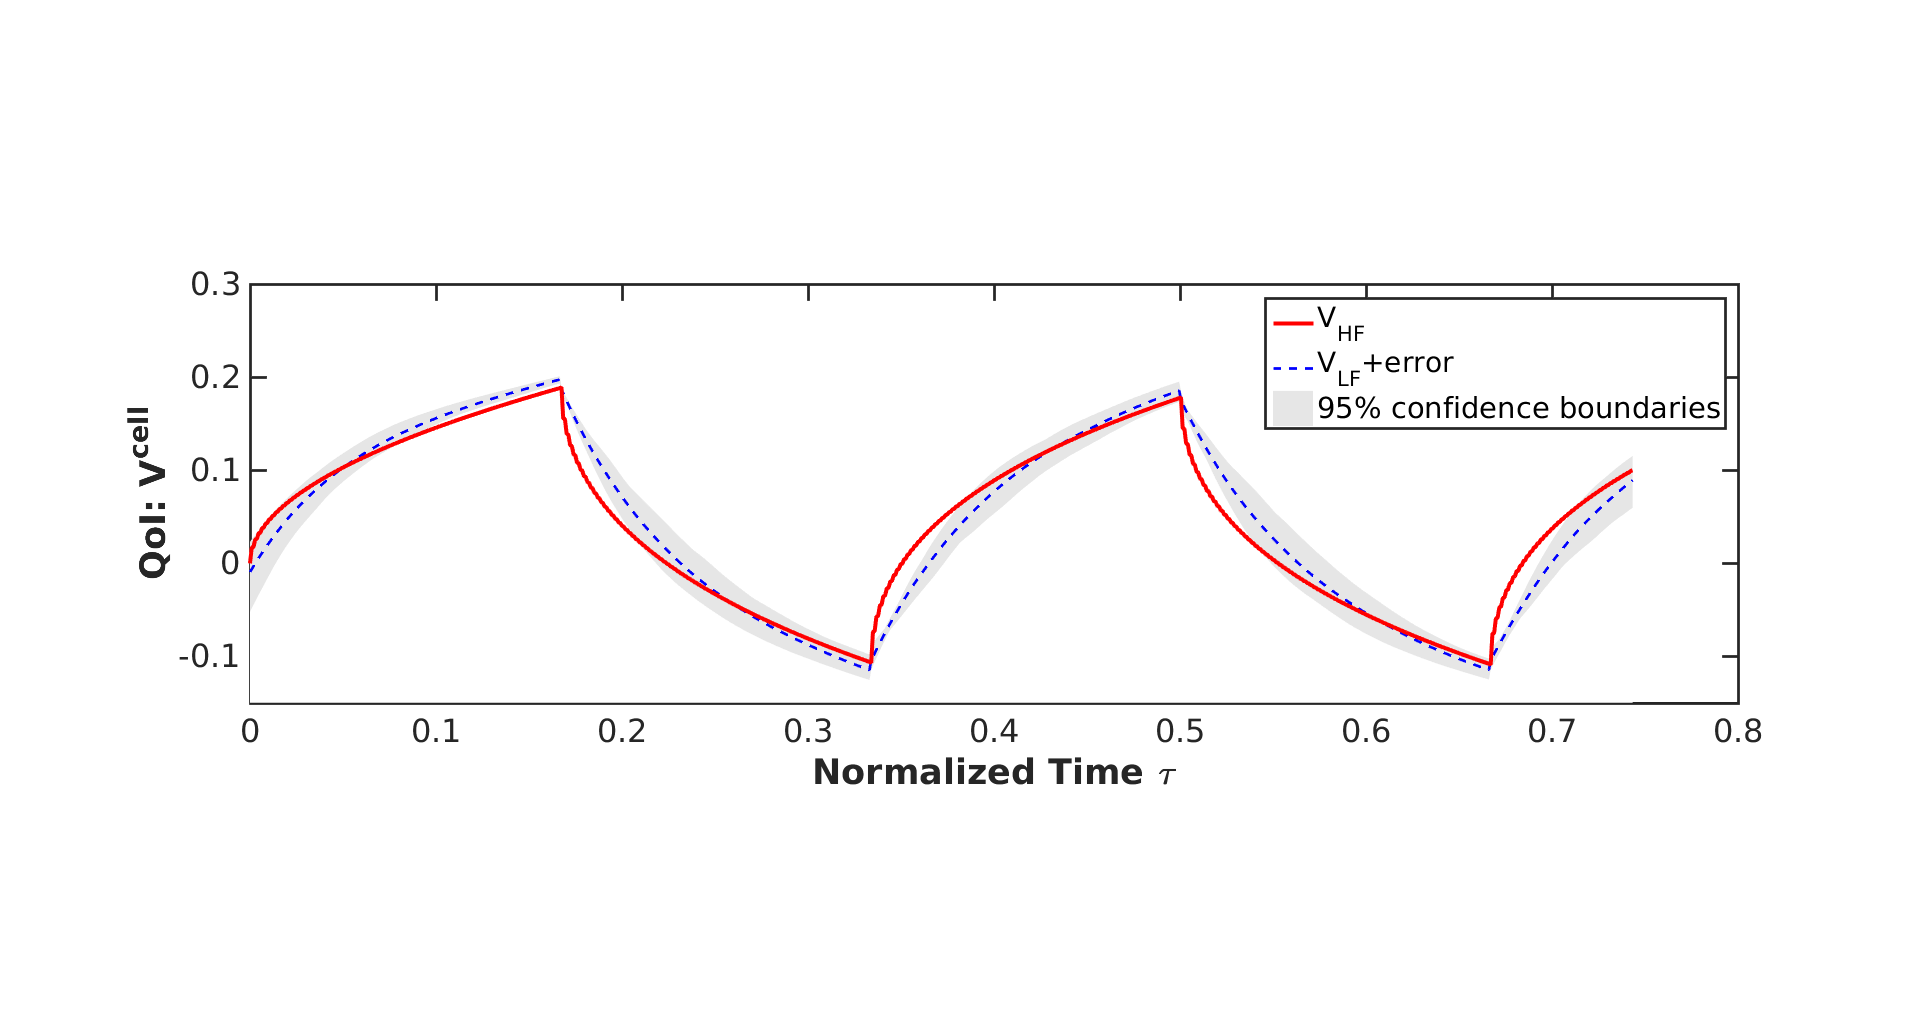
\includegraphics[trim = 1.3in 2.2in 1.6in 2.8in, clip, width=1\textwidth]{figs_report/V_bound.png} 
\end{figure}
\end{center}
\end{column}
\end{columns}
\vspace{2mm}

\vfill
\end{frame}


%===============================================================================
% Slide 3
%===============================================================================
\begin{frame}
\frametitle{Model Inadequacy}
\vfill

\begin{columns}
\begin{column}{.50\textwidth}
%-----------------------------
\begin{block}{}
\begin{itemize}

\item The equivalent circuit models and transmission lines are not able to fully capture the behavior of real supercapacitors. 

\item The high-fidelity 3D finite element model makes it possible to understand better how physical electrochemistry and other design parameters affects super capacitor behavior.  But this comes at a cost of complex operation mode with high performance computing requirement.  

\item Similar procedure will be pursue to formulate inadequacy of the 1D model with respect to finite element 3D model.

\item The 1D model enhanced with stochastic inadequacy representation, can be utilized to provide low cost computational predictions for analyzing electrochemical impedance spectroscopy data, computing heat production in thermal analysis, etc. 

\end{itemize}

\end{block}
\end{column}
%====================
\begin{column}{.42\textwidth}
\begin{center}
%\vspace{-4mm}
\begin{figure}[h]
    \centering
    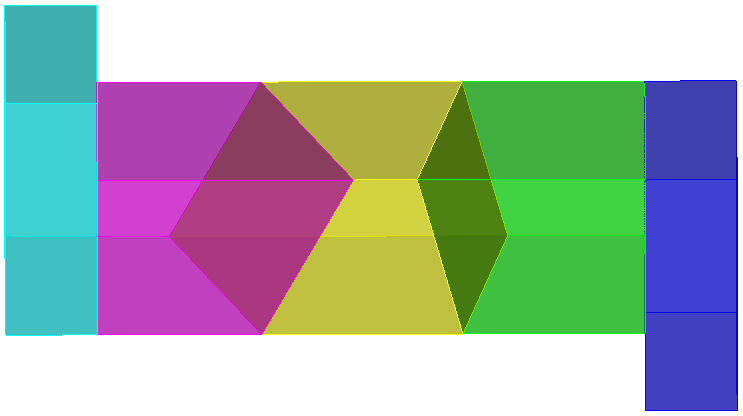
\includegraphics[trim = 0in 0in 0in 0in, clip, width=0.8\textwidth]{figs_report/transparent.png} 
    \\{3D finite element mesh of supercapacitor$^1$.}\\
    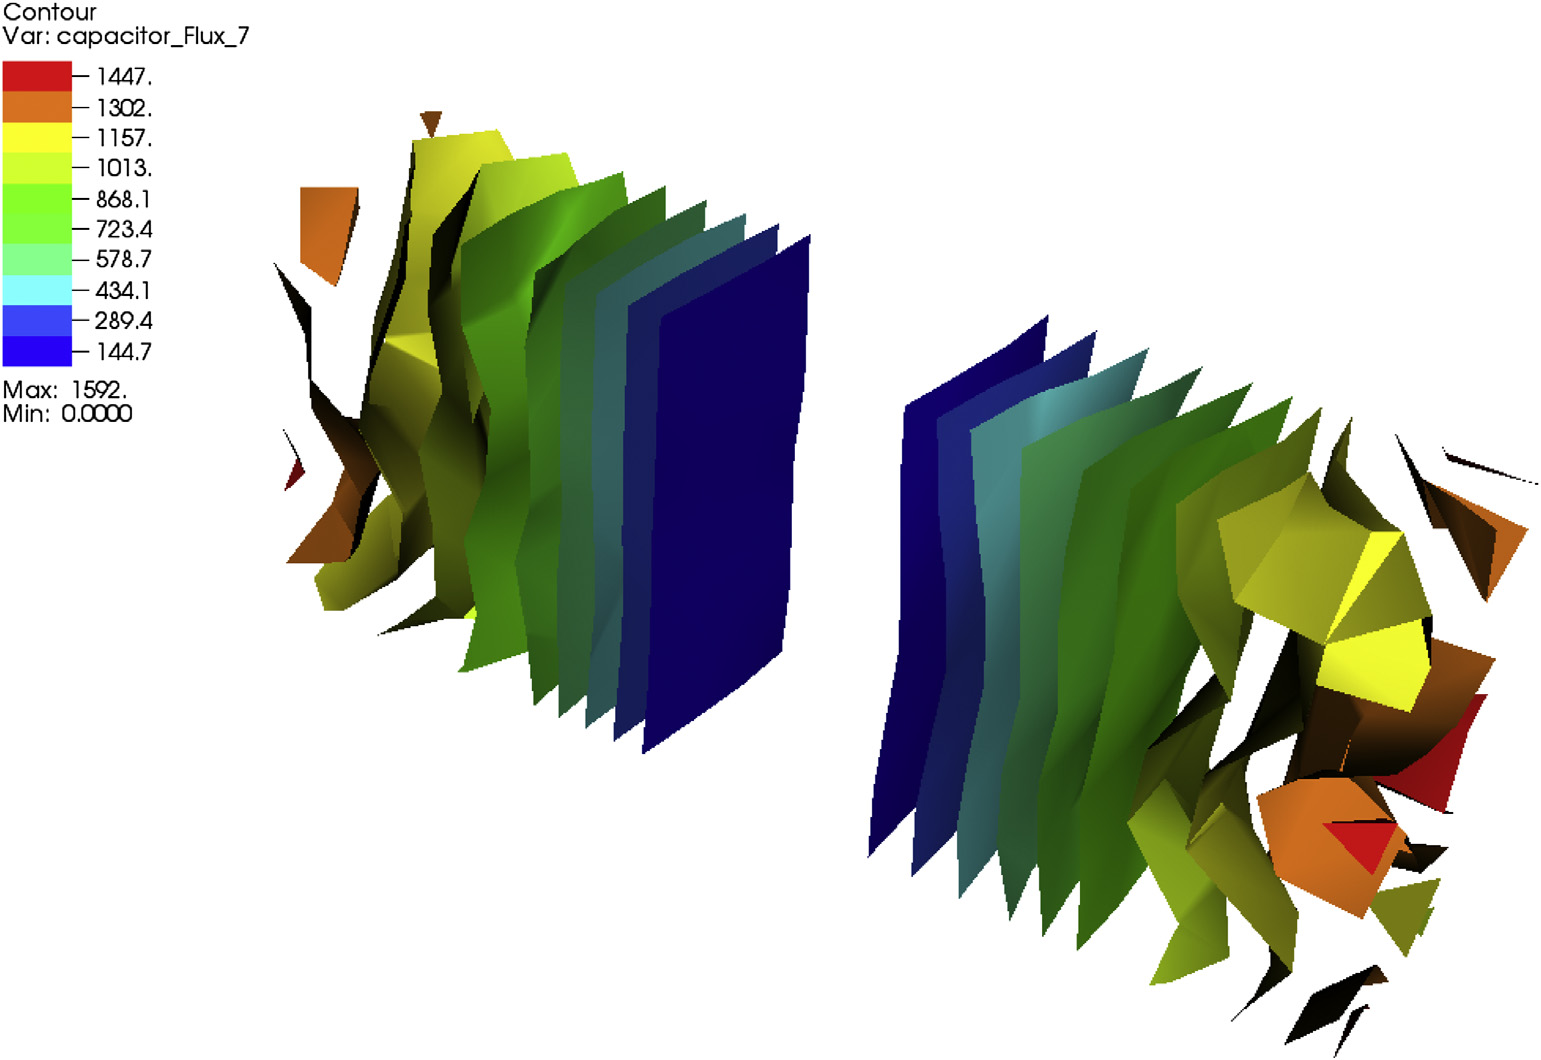
\includegraphics[trim = 0in 0in 0in 0in, clip, width=0.8\textwidth]{figs_report/parallel_conf.png}
    \\ {Spatial distribution of the current density for parallel plate supercapacitor configuration$^2$.}
\end{figure}
\end{center}
\end{column}
\end{columns}

\vspace{0.1in}
\noindent\rule{5cm}{0.4pt}\\
\begin{footnotesize}
$^1$ Lebrun-Grandie and Turcksin. \textit{Cap: C++ library for modeling energy storage devices}. ORNL-CEES.

$^2$ Allu, Velamur Asokan, Shelton, Philip, Pannala. \textit{Journal of Power Sources} 256 (2014): 369-382.
\end{footnotesize}

\vfill
\end{frame}






\end{document}

